
\documentclass[a4paper,useAMS,usenatbib]{mnras}

\usepackage{graphicx}
\usepackage{setspace}
\usepackage{natbib}
\usepackage{color}
\usepackage{amsmath,amssymb}
\usepackage{times}
%\usepackage{aas_macros}
\usepackage{hyperref}


%\voffset-.4in

%\AtBeginShipout{%
%  \ifnum\value{page}>1 %
%    \typeout{* Additional boxing of page `\thepage'}%
%    \setbox\AtBeginShipoutBox=\hbox{\copy\AtBeginShipoutBox}%
%  \fi
%}


\bibliographystyle{mnras}

%%%%%%%%%%%%%%%%%%%%%%%%%%%%%%%%%%%%%%%%%%%%%%%%%%%%%%%%%%%%%%%%%%%%%%%%%%%%%

\newcommand{\Gaia}{{\it Gaia}}
\newcommand{\gaia}{\textit{Gaia} }

%%%%%%%%%%%%%%%%%%%%%%%%%%%%%%%%%%%%%%%%%%%%%%%%%%%%%%%%%%%%%%%%%%%%%%%%%%%%%

\title[Orphan Stream in \gaia DR2]{Piercing the Milky Way. Orphan
  Stream in \gaia DR2}

\author[OATs]{OATs: Orphan Aspen Treasury\\
  $^{1}$Institute of Astronomy, Madingley Rd, Cambridge, CB3 0HA\\
  $^{2}$Center for Computational Astrophysics, Flatiron Institute, 162 5th Avenue, New York, NY 10010, USA\\
  $^{3}$Department of Physics, University of Surrey, Guildford GU2 7XH, UK\\
}

\begin{document}

\maketitle

\label{firstpage}

\begin{abstract}
We use astrometry and broad-band photometry from Data Release 2 of the
ESA's Gaia mission.

\end{abstract}

\begin{keywords}
Milky Way -- galaxies: dwarf -- galaxies: structure -- Local Group -- stars
\end{keywords}

\section{Introduction}



%
\begin{figure*}
  \centering
  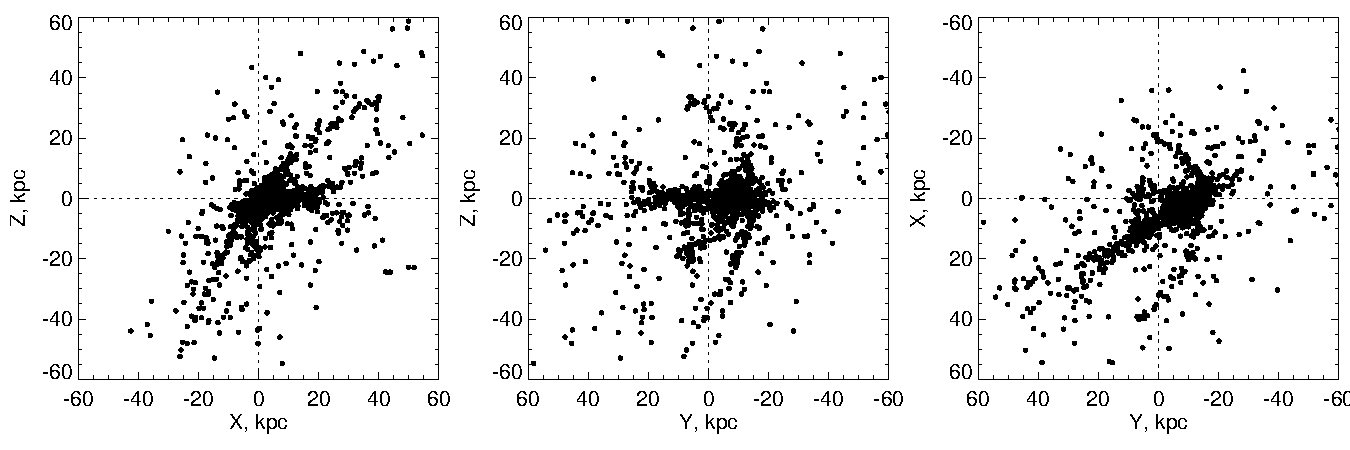
\includegraphics[width=0.95\textwidth]{orphan_paper_xyz.pdf}
  \caption[]{Galacto-centric distributions of the $\sim1,500$ \gaia
    DR2 RR Lyrae stars projected close to the OS on the sky. Only
    stars with $|\phi_2|<4^{\circ}$ and $-300<v_l <-100$, $-300<v_b
    <300$ are shown. {\it Left:} $X,Z$ plane. {\it Middle:} $Y,Z$
    plane. {\it Right:} $X,Y$ plane. Note a prominent, narrow and long
    stream-like over-density visible in all three panels.}
   \label{fig:xyzgdr2}
\end{figure*}
%

It so happened that the most striking example of a nearby binary
interaction was only just being discovered at the time of the writing
of \citet{Toomre1972} and hence could not be included in their
analysis. \citet{Wannier1972} and \citet{Kuilenburg1972} detected long
streams of HI in the Southern sky, and some two years later these were
shown to connect to the Magellanic Clouds by
\citet{Mathewson1974}. The Magellanic Stream (MS, as it is known
today) has since been mapped across the sky \citep[see
  e.g.][]{Putman2003,Nidever2008,Nidever2010} and is today
unambiguously demonstrated to have originated in the interaction
between the Large and the Small Clouds \citep[LMC and
  SMC,][]{Besla2007, Besla2010, Diaz2011, Diaz2012}. While the stellar
counterpart to the MS is yet to be discovered, the last two years have
seen a marked increase in the number of reported detections of low
surface-brightness stellar sub-structure in the vicinity of the Clouds
\citep[see
  e.g.][]{Mackey2016,Belokurov2016,Belokurov2017,Deason2017,Pieres2017,Mackey2018,Nidever2018}. In
particular, \citet{Mackey2016,Mackey2018} concentrate on the
perturbations in and around the LMC's stellar disc. They uncover a
wealth of sub-structure, some of which (such as the long stream-like
feature in the North of the LMC) they tentatively attribute to the
tidal influence of the MW \citep[][]{Mackey2016}. They also
detect prominent stellar debris over-densities in the Southern parts
of the LMC and put forward two formation scenarios: one to do with the
disruption of the LMC's disc and one linked to the episodic stripping
of the SMC \citep[see also][who argued for the importance of repeated
  interactions with the SMC]{besla_etal_2016}.

%
\begin{figure*}
  \centering
  \includegraphics[width=0.9\textwidth]{orphan_paper_selection.pdf}
  \caption[]{OS member selection. {\bf SK to provide details}}
   \label{fig:selection}
\end{figure*}
%


%
\begin{figure*}
  \centering
  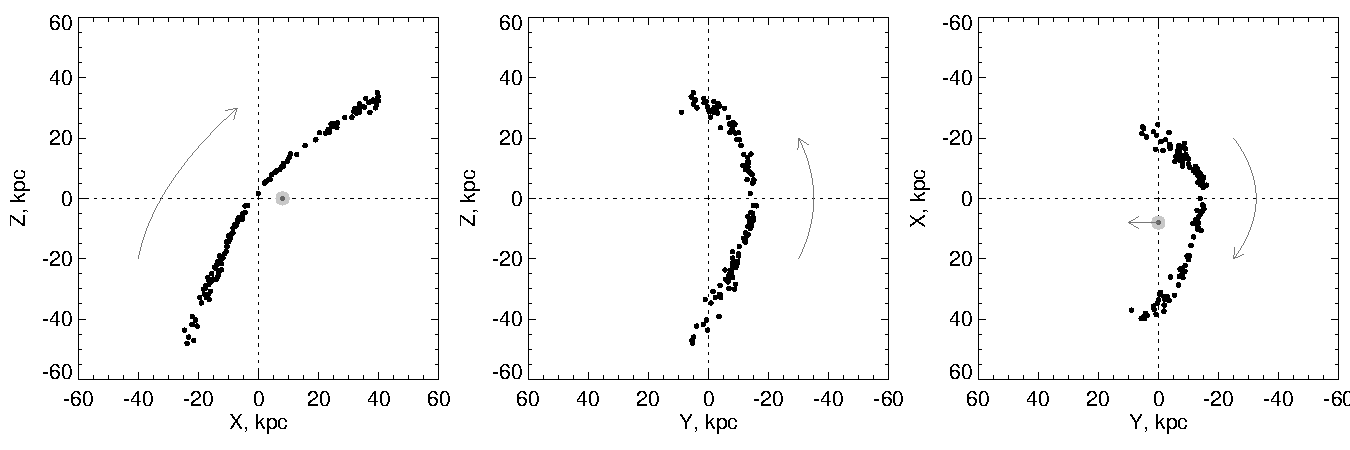
\includegraphics[width=0.97\textwidth]{orphan_paper_xyz_members.pdf}
  \caption[]{Companion of Figure~\ref{fig:xyzgdr2}. Here only the
    likely OS members (see Figure~\ref{fig:selection} and main text
    for details) are shown in Galacto-centric coordinates.}
   \label{fig:xyzmem}
\end{figure*}
%

In this Letter, we use a combination of Gaia's (Data Release 2, or
GDR2) photometry and astrometry to produce an uninterrupted panorama
of the Magellanic Clouds. We focus on the density fluctuations between
10 and 30 degrees away from the LMC's centre. While our maps do not
attain the same level of detail achievable using deep imaging with
instruments such as DECam, they help to fill in the gaps in the
Magellanic puzzle. Moreover, Gaia's astrometry has the
unprecedented power to remove the bulk of the intervening MW's
disc population and thus extend the study of the Clouds to regions
not accessible even with the deepest imaging surveys.

%Specifically, we demonstrate that two long and narrow tidal arms exist
%in the Northern and Southern outskirts of the LMC's disc, most likely
%produced as a result of the combined effect of the MW tides and the
%interaction with the SMC during its most recent passage near the Large
%Cloud.

\section{Orphan Stream with \gaia DR2 RR Lyrae}

We select a high-purity all-sky sample of RR Lyrae candidate stars
from two separate source catalogues released as part of the \gaia DR2
\citep[][]{Prusti2016, Brown2018}. More precisely, tables
\texttt{vari\_classifier\_result} and \texttt{vari\_rrlyrae}
\citep[see][]{Clementini2018,Holl2018} are joined, removing the
duplicates, and the stellar astrometry and photometry are obtained
from the main \texttt{gaia\_source} catalogue. We have culled
potential interlopers requiring \textit{phot\_bp\_rp\_excess\_factor}
to be less than 3 and have assumed $A_G=2.27$ and $M_G=0.64$ for the
extinction coefficient and the RRL absolute magnitude in the \Gaia's
$G$ band respectively \citep[see][for further
  details]{Iorio2018}. Additionally, we have assumed the Sun's
distance from the Galactic center of 8 kpc, the Local Standard or Rest
(LSR) of 235 km s$^{-1}$ and the Sun's peculiar motion as given in
\citet{LSR}.

To select the likely OS members, we translate the stellar celestial
coordinates in equatorial system $\alpha, \delta$ into a new
coordinate system $\phi_1, \phi_2$ aligned with the stream \citep[see
  e.g.][]{Koposov2010}. More specifically, based on the OS detections
reported in \citet{OS_V, OS_C, Newberg2010}, we use a great circle
with a pole at $(\alpha_{\rm OS}, \delta_{\rm OS})=(70.5^{\circ},
-13^{\circ})$. The origin of this stream's coordinate system is chosen
to be at $(\alpha_0, \delta_0)=(188^{\circ}, -63^{\circ})$, near the
position of the OS's crossing of the Galactic disc. Several attempts
at the OS kinematic characterization can be found in
\citet{Newberg2010} and \citet{Sohn2016}. Given the OS's line-of-sight
velocity and the HST-based proper motions, we notice that the stream's
velocity component along the Galactic longitude $v_l$ remains negative
irrespective of the debris position on the sky, i.e. the stream is in
prograde motion with respect to the Galactic rotation. Accordingly, we
explore the distribution of the possible OS members selected with the
following simple cuts.

%
\begin{equation}
  \begin{aligned}
    |\phi_2| &< 4^{\circ}\\
    -300<v_l &<-100\\
    -300<v_b &<300
  \end{aligned}
\end{equation}
%

Figure~\ref{fig:xyzgdr2} shows the distributions of $\sim$1,500 RRL
stars selected with the above cuts in Galacto-centric coordinates
$X,Y$ and $Z$; here $X$ points to the Galactic anti-center and the Sun
is at $(X,Y,Z)=(8,0,0)$. A long and narrow arc or RRL stars is visible
in all three projections, crossing the Galaxy from the North (where it
is seen at $Z>0$ and $X>0$) to the South (where the signal is ar $Z<0$
and $X<0$). The stream spans a gigantic $\sim$100 kpc, traveling in
almost uninterrupted fashion through the Milky Way, coming as close as
$\sim$15 kpc to its center and reaching as far as $\sim$50 kpc into
the halo. While the Northern portion of the stream had been seen
before with SDSS and PS1, the view of its Southern Galactic section
uncovered here with \gaia DR2 is entirely new.

We can further clean the OS membership by looking closely at the
behavior of the RRL stars close to the equator of the stream's
coordinate system. To this end, Figure~\ref{fig:selection} shows the
distribution of RR Lyrae as a function of the along-stream coordinate
$\phi_2$. As the top panel of the Figure illustrates, the stream spans
some $\sim200^{\circ}$ in $\phi_1$ while exhibiting a slight bend of
several degrees in $\phi_2$. The heliocentric distance of the Orphan
debris changes slowly within $-50^{\circ}<\phi_1<50^{\circ}$, but
beyond that, the stream appears to shoot rapidly to large distances,
reaching $\sim50$ kpc on either end. Finally, a clear kinematic
pattern is visible in the bottom panel of Figure~\ref{fig:selection},
where the stream $\mu_{\phi,1}$ proper motion arches up to $\sim$4 mas
year$^{-1}$ around $\phi_1\sim40^{\circ}$ from values close to $\sim0$
mas year$^{-1}$ near the tips of the stream. Note that in all three
projections, the width of the stream also changes as a function of
$\phi_1$. Some of this variation may be due to the intrinsic evolution
of the debris density along the stream \citep[see e.g.][]{stray}, but
much of it may plausibly be associated with the change in the
measurement quality. As the stream moves away from the Sun at high
values of $|\phi_1|$, the associated errors in distance and proper
motion grow quickly, increasing the scatter around the stream's
centroid. 

Each panel of Figure~\ref{fig:selection} shows a sample of stars
selected after applying the polynomial masks from the other two panels
(the masked areas are highlighted in pale blue in each panel). The
boundaries of the masks are chosen to wrap around the bulk of the
stream's debris in a smooth and continuous manner. More precisely, the
masks are drawn as follow {\bf SK to explain}. The parameters of the
polynomials used for the stream selection are given in table XXX. {\bf
  SK to supply}. Applying all three masks shown in the Figure yields
the total of NNN OS candidate members. Table YYY lists all RRL stars
identified using the procedure described above together with their
positional and kinematic measurements from GDR2. {\bf Table
  needed}.

Figure~\ref{fig:xyzmem} is a companion to Figure~\ref{fig:xyzgdr2} as
it also shows the Galacto-centric positions of the \gaia RR Lyrae
stars, but now only those selected using the masks described
above. Left panel of the Figure emphasizes the high eccentricity of
the OS as the stream appears high stretched in this
projection. Noticeable in the middle and right panels of the Figure is
the change in the stream's curvature between the Southern and the
North Galactic hemispheres. The view of the OS in other phase-space
projections can be found in Figure~\ref{fig:memother}.

Top left panel of the Figure presents the on-sky positions of the
likely OS members in the stream-aligned coordinate system. Immediately
apparent is the striking change of the stream curvature around
$\phi_1\sim20^{\circ}$ - immediately after the stream re-emerges after
passing through the Galactic disc - where the debris behavior changes
from gently slopping down to sharply rising up in
$\phi_2$. Additionally, in the Northern end of the stream, at
$\phi_1\sim100^{\circ}$ there appears to be a curious hook
downwards. There exists a corresponding change in the debris
kinematics. For example, proper motion components $\mu_{\alpha}$ and
$\mu_{\delta}$ also show a switch in the gradient as a function of
$\phi_1$ around $\phi_1\sim20^{\circ}$. Note, however that the
evolution of the physical velocity components $v_l$ and $v_b$ (and
also $v_{\phi,1}$ and $v_{\phi,2}$) is considerably
smoother. Therefore, some of the change in the proper motions (shown
in the second row from the top) is due to the change in the
line-of-sight distance.

%
\begin{figure*}
  \centering
  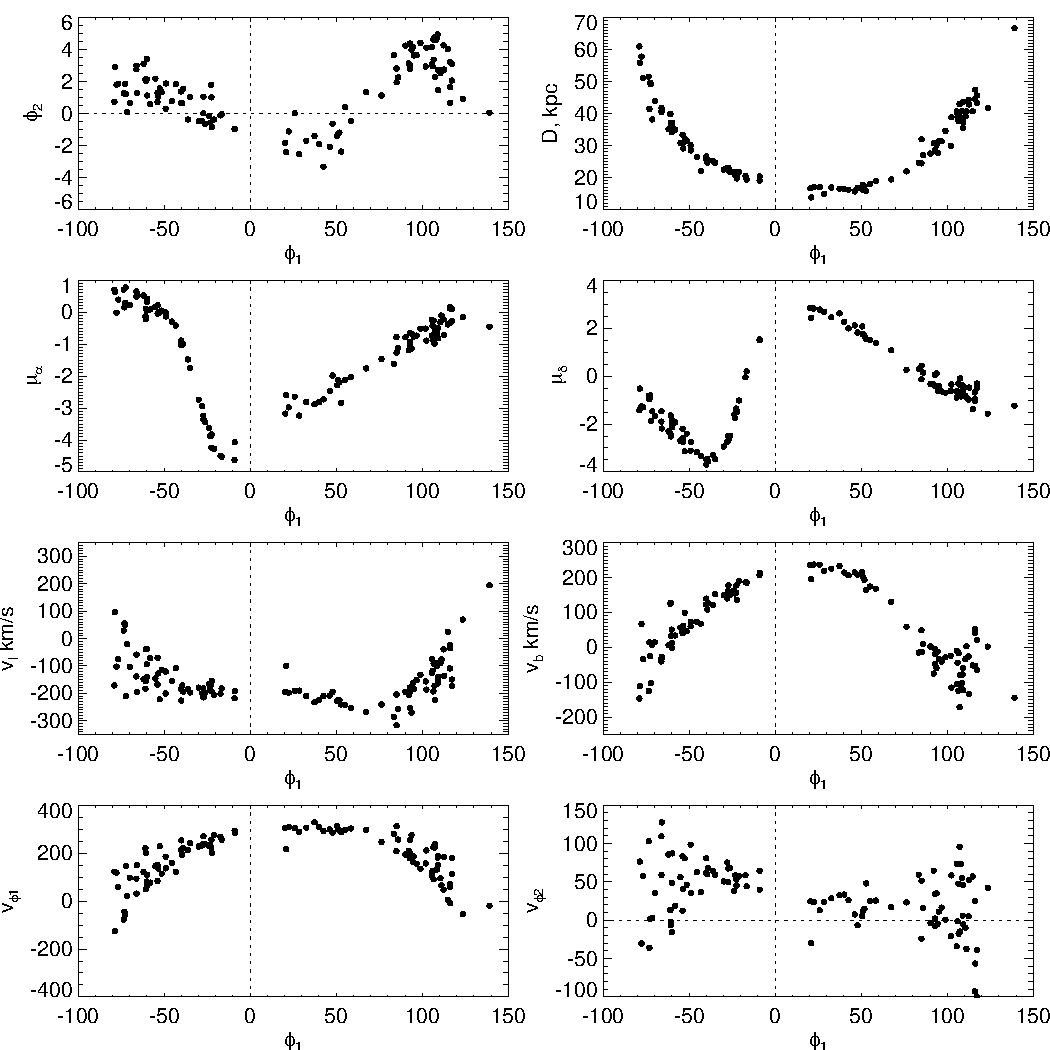
\includegraphics[width=0.9\textwidth]{orphan_paper_phi1_members.pdf}
  \caption[]{Phase-space projections of the likely OS member RR Lyrae
    as a function of the stream longitude $\phi_1$. {\it Top left:}
    Positions of the OS stars on the sky in the stream-aligned
    coordinates $\phi_1, phi_2$. {\it Top right:} Heliocentric
    distance as a function of $\phi_1$. {\it Second row, left:} RA
    component of proper motion $\mu_{\alpha}$. {\it Second row,
      right:} Dec component of proper motion $\mu_{\delta}$. {\it
      Third row, left:} Velocity component along Galactic longitude
    $v_l$. {\it Third row, right:} Velocity component along Galactic
    latitude $v_b$. {\it Bottom left:} Along-stream velocity
    $v_{\phi,1}$. {\it Bottom right:} Across-stream velocity
    $v_{\phi,2}$.}
   \label{fig:memother}
\end{figure*}
%

\section{OS with giants in \gaia and DECaLS}

In order to investigate how the MW and SMC affect the LMC's disc and
whether they can induce the spiral features shown in Figure
\ref{fig:map}, we have run a series of simulations in the spirit of
\cite{Toomre1972}. In particular, we simulate the disc of the LMC as a
series of particles in concentric rings which are initially on
circular orbits. While this ignores the initial non-circular motions,
it captures the overall behavior of the disc over the relatively short
timescales considered here. The system is then evolved in the presence
of the MW and the SMC. We model the LMC's potential as a Hernquist
profile \citep{hernquist_profile} which satisfies the rotation curve
measurement at a radius of 8.7 kpc from \cite{vandermarel_lmc} (for
each LMC mass, the scale radius is fixed by this constraint). The
initial orientation and rotation sense of the LMC are chosen to match
the observations from \cite{vandermarel_lmc}. The SMC is also modelled
as a Hernquist profile satisfying the rotation curve measurement at a
radius of 3 kpc from \cite{staminirovic_smc_mass}. The MW is modelled
as the 3-component potential, \texttt{MWPotential2014}, from
\cite{galpy}. Starting from their present day positions, the LMC and
SMC are rewound for 1 Gyr (in the presence of each other and the MW),
at which point particles are placed on circular orbits around the
LMC. For each simulation, we place 5000 particles on 50 separate
concentric circles with radii evenly spaced from 1 to 20 kpc. The
simulation is then evolved to the present. For the LMC's present day
position and velocity, we use a distance of $49.97 \pm 1.126$ kpc
\citep{pietrzynski_lmc_dist}, a radial velocity of $-262.2\pm3.4$ km/s
\citep{vandermarel_lmc_rv}, and PMs of $(\mu_\alpha \cos \delta,
\mu_\delta) = (1.91\pm 0.02,0.229\pm0.047)$ mas/yr
\citep{kallivayalil_lmc_pm}. For the SMC, we use a distance of
$62.1\pm1.9$ kpc \citep{graczyk_smc_distance}, a radial velocity of
$145.6\pm0.6$ km/s \citep{harris_smc_vel}, and PMs of $(\mu_\alpha
\cos \delta, \mu_\delta) = (0.772\pm 0.063,-1.117\pm0.061)$ mas/yr
\citep{kallivayalil_lmc_pm}. For each choice of the LMC and SMC masses
and scale radii, we sample their present day position and velocity and
simulate 100 realizations to explore the variety of outcomes.

In Figure \ref{fig:sim_multi} we isolate the effect of the MW
(left-most column) and the SMC (middle two columns) on the LMC. The
two rows show two different realizations of the LMC and SMC's present
day position and velocity. The top row shows an LMC with a closer
encounter with the SMC ($r_{\rm peri} \sim 10$ kpc), while the bottom
row shows a more distant encounter ($r_{\rm peri} \sim 15$ kpc). The
tidal field of the MW is primarily responsible for bending the
Northern half of the LMC, similar to what was found in $N$-body
simulations in \cite{Mackey2016}, and creates a spiral arm feature
similar in position and orientation to what it seen in the data. The
SMC can create one or two spiral arms, depending on how strong of an
interaction it has with the LMC during its most recent
pericenter. While this is in seeming contradiction to the results of
\cite{Toomre1972}, we stress that we are observing the LMC disc only
$\sim 150$ Myr after its most recent passage with the SMC and that it
takes time for the spiral features to form. If the LMC was simulated
for longer, the second spiral would form in the lower panel of Figure
\ref{fig:sim_multi}. Interestingly, we find that the SMC creates a
strong spiral arm in the South which matches the observed Southern
stream. We found that changing the SMC mass from $5\times 10^9
M_\odot$ to $10^{10} M_\odot$ resulted in only a modest change in the
spiral features. Our simulations do not contain the ``claw''-like
features visible in the data in the Southern parts of the LMC. We
conjecture that these density features are remnants of much earlier
interactions between the two Clouds. The fourth column of the figure
shows the effect of both the MW and the SMC. This
demonstrates that their combined effect is needed to create the two
spirals observed in the LMC. It also illustrates how a close encounter
with the SMC can truncate the Western portion of the LMC's disc (top,
second from the right panel) similar to what it seen in the
data. Taken together, this shows that morphology of the LMC's disc and
the associated spiral structure can be used to reveal its rich
dynamical history.

In a similar vein, we also explore the effect of the LMC's mass on its
morphology in Figure \ref{fig:sim_multi}. While the first four columns
show a $2\times 10^{10}M_\odot$ LMC, the final column shows a $2\times
10^{11} M_\odot$ LMC.  Note that the final column should be compared
with the fourth column since these have the same setup.  As the LMC
mass is increased, we find that the LMC is deformed less by the
MW. This is because the increased LMC mass results in a larger tidal
radius and hence a larger region where the effect of the MW is
negligible. Interestingly, only the lowest mass LMC we consider
($2\times 10^{10} M_\odot$) can match the tightly wound spiral seen in
the North (see Fig. \ref{fig:map}). Since this mass is only slightly
higher than the mass constraint within 8.7 kpc from
\cite{vandermarel_lmc}, this could suggest that the LMC has already
been significantly stripped. However, we stress that these simulations
are only meant to be the first step in showing that the morphology
(including spirals) of the LMC's disc can provide useful constraints
on the properties of the LMC, SMC, and on the tidal effect of the
MW. With this aim in mind, the rich PMs in Figure
\ref{fig:vel} will also be useful in future modelling efforts.

In summary, we have used the exquisite data from Gaia DR2 to
unveil a global view of the perturbations to the LMC's disc. In
particular, there are two clear spiral features, as well as some complex
substructure to the South of the LMC (see Fig. \ref{fig:map}). While
some of this structure was seen before
\citep[e.g.][]{Mackey2016,Mackey2018}, the uninterrupted view afforded
by Gaia allows us to better understand how these features
arose. We simulated the combined effect of the MW and SMC on
the LMC's disc and found that both are important for creating the
spiral features seen in the data. Namely, the MW is responsible
for deforming the Northern part of the LMC while the most recent
passage of the SMC creates the strong spiral feature in the South. A
close passage with the SMC can also truncate the Western side of the
LMC's disc. Finally, we showed that the distant Magellanic Red
Giants detected here can be used to map out the LMC's mass distribution at
unprecedentedly large distances.

\section*{Acknowledgments}

We thank Michael for illuminating discussions. The research leading to
these results has received funding from the European Research Council
under the European Union's Seventh Framework Programme (FP/2007-2013)
/ ERC Grant Agreement n. 308024. This research was started at the NYC
Gaia DR2 Workshop at the Center for Computational Astrophysics of the
Flatiron Institute in April 2018 and made use of data from the
European Space Agency mission Gaia (http://www.cosmos.esa.int/gaia),
processed by the Gaia Data Processing and Analysis Consortium (DPAC,
http://www.cosmos.esa.int/web/gaia/dpac/consortium). Funding for the
DPAC has been provided by national institutions, in particular the
institutions participating in the Gaia Multilateral Agreement.

\bibliography{references}

\label{lastpage}

\end{document}

